\label{sec:ndsResults}
%\subsection{Проблемы проектирования}

С помощью построенной в комплексе ``Conver'' расчетной МКЭ-модели были проведены прочностные исследования напряженно-деформированного состояния(НДС) модели гипотетического БПЛА, в которой толщины всех стенок и панелей были приняты равными $1\text{мм}$ (минимальная из существующего сортамента толщина алюминиевых панелей). На основе полученных данных была проведена оптимизация толщин панелей и стенок отсеков для нахождения минимальной по весу конструкции, удовлетворяющей требованиям прочности.

Для полученной модели можно выделить следующие особенности НДС:

\begin{enumerate}
\item Усилия в обшивке фюзеляжа малы за исключением обшивки центроплана. Т.о. большую часть обшивки можно выполнять по условию технологических ограничений на минимальных толщинах.
\item Наибольшие усилия наблюдаются в фюзеляжной части центроплана и в корне крыла. Так, в корне крыла наблюдаются следующие величины усилий: $Q = 13,7~\text{тс}$, $M_\text{изг} = 80~\text{тс}\cdot\text{м}$. 
\item Значительные усилия наблюдаются на стенках отсека двигателя в местах крепления двигателя (дополнительный анализ этой особенности произведен далее в данном разделе). На Рис.\ref{fig:WingDeformation3},\ref{fig:WingRotating} показаны эпюры изгиба и кручения крыла. 
\end{enumerate}  

Общая картина НДС расчетной модели БПЛА представлена на Рис.\ref{fig:patranRearDeformed}--\ref{fig:patranTopIsoWithoutSk}


\begin{figure}[H]
\centering

\captionsetup{justification=centering}
\def\svgwidth{0.9\textwidth}
\input{figures/WingDeformation3.pdf_tex}
\caption{Эпюры прогибов лонжеронов, полученные в результате расчетов МКЭ- и балочной моделей}
\label{fig:WingDeformation3}
\end{figure}

\begin{figure}[H]
\centering
\def\svgwidth{0.9\textwidth}
\input{figures/WingRotating.pdf_tex}
\caption{Кручение крыла. Разность прогибов лонжеронов}
\label{fig:WingRotating}
\end{figure}


\begin{figure}[H]
\centering
\includegraphics[width=0.8\textwidth]{patran/rear_deformed}
\caption{Вид сзади, деформированное состояние конструкции гипотетического БПЛА}
\label{fig:patranRearDeformed}
\end{figure}


\begin{figure}[H]
\centering
\includegraphics[width=0.7\textwidth]{patran/bottom}
\caption{Вид снизу}
\label{fig:patranBottom}
\end{figure}


\begin{figure}[H]
\centering
\includegraphics[width=0.7\textwidth]{patran/top}
\caption{Вид сверху}
\label{fig:patranTop}
\end{figure}


\begin{figure}[H]
\centering
\includegraphics[width=0.8\textwidth]{patran/bottom_iso}
\caption{Вид в изометрии снизу}
\label{fig:patranBottomIso}
\end{figure}

\begin{figure}[H]
\centering
\includegraphics[width=0.8\textwidth]{patran/bottom_iso_noskin}
\caption{Вид снизу в изометрии без обшивки}
\label{fig:patranBottomIsoWithoutSkin}
\end{figure}

\begin{figure}[H]
\centering
\includegraphics[width=0.8\textwidth]{patran/bottom_zoom}
\caption{Вид на стык крыла с фюзеляжем снизу в изометрии}
\label{fig:patranBottomIsoZoom}
\end{figure}


\begin{figure}[H]
\centering
\includegraphics[width=0.8\textwidth]{patran/top_iso}
\caption{Вид сверху в изометрии}
\label{fig:patranTopIso}
\end{figure}

\begin{figure}[H]
\centering
\includegraphics[width=0.8\textwidth]{patran/top_iso_noskin}
\caption{Вид сверху в изометрии без обшивки}
\label{fig:patranTopIsoWithoutSk}
\end{figure}
 \subsection{Крепление хвостовой части к кессону центроплана} 
\label{sec:pants}
\begin{figure}[H]
\centering
\includegraphics[width=0.6\textwidth]{IsoviewOfPantsBW}
\caption{Вид центральной части фюзеляжа с выделенными стенками}
\label{fig:IsoviewOfPants}
\end{figure}

Для предварительной оценки НДС наиболее нагруженных деталей и узлов хвостовой части корпуса БПЛА была решена модельная задача по оценке нагруженности вертикальных стенок, обеспечивающих передачу нагрузок от двигателя, оборудования и топлива на конструкцию центроплана (стенки обозначены на Рис.~\ref{fig:IsoviewOfPants} серой заливкой, светло-серой заливкой обозначены зоны основных узлов крепления двигателя). Уровень нагружения был оценен на основе аналитических формул. Схема нагружения модельных стенок показана на Рис.\ref{fig:IsoviewOfPantsModel}.

\begin{figure}[H]
\centering
%\def\svgwidth{0.9\textwidth}
\input{figures/IsoviewOfPantsModel.pdf_tex}
\caption{Схема нагружения модельных стенок}
\label{fig:IsoviewOfPantsModel}
\end{figure}

%
%\begin{figure}[H]
%\centering
%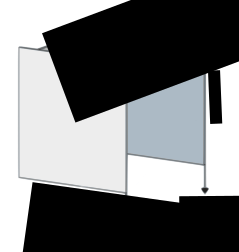
\includegraphics[width=0.8\textwidth]{IsoviewOfPantsModel}
%\caption{Схема нагружения модельных стенок}
%\label{IsoviewOfPantsModel}
%\end{figure}


Уровень нагружения оценивался по величинам касательных напряжений. Касательные напряжения в пластине при чистом сдвиге равны

\begin{equation}
\tau=\frac{3}{2}\cdot\frac{Q}{bh}
\end{equation}
Критические по устойчивости касательные напряжения в пластине при чистом сдвиге равны \cite{Volmir}:

\begin{equation}
\tau_\text{кр}=\frac{K}{12}\frac{\pi^2D}{b^2h} = \frac{K}{12}\frac{\pi^2E}{(1-\mu^2)}\left(\frac{h}{b}\right)^2,\, K=5.34 + 4\frac{a}{b},
\end{equation}
где $a$ - размер пластины вдоль направления действия силы, $b$ - размер пластины поперек направления действия силы, $h$ - толщина пластины, $D$ - изгибная жесткость пластины, $E$ - модуль Юнга, $\mu$ - модуль Пуассона материала пластины, $Q$ - приложенная сила.
Допускаемые толщины найдем из условия

\begin{equation}
\tau_\text{кр} \geq \tau \to h \geq \sqrt[3]{\frac{3\cdot12}{2}\frac{Qb\cdot(1-\mu^2)}{k\pi^2E}} 
\end{equation}
Подставляя значения, получим:

\begin{equation}
Q=\frac{8000}{n}\text{кгс},\,a=1300\text{мм},\,b=1009\text{мм},\,\mu=0.3,\,E=7000\frac{\text{кгс}}{\text{мм}^2}
\end{equation}

\begin{equation}
h \geq \sqrt[3]{\frac{18\cdot8000\cdot1000\cdot(1-\mu^2)}{k\pi^2En}} = \frac{5.67}{\sqrt[3]{n}} 
\end{equation}

Таким образом, для случаев $n = 2$ и $n = 4$  были получены минимальные допустимые толщины, 
равные

\begin{equation}
h\geq4.50\text{мм},\,n=2
\end{equation}
\begin{equation}
h\geq2.83\text{мм},\,n=4
\end{equation}
%\subsubsection{Фюзеляжная часть центроплана}

Другим проблемным местом была фюзеляжная часть центроплана. Из-за требований компоновки, а именно интеграции двигателя, центроплан необходимо делать изогнутым (Рис.\ref{fig:centroplan}). Это вносит дополнительные трудности в виде увеличения веса по сравнению с прямым центропланом. Исследованию фюзеляжной части центроплана (выделена серым на Рис.\ref{fig:centroplan}) посвящена глава \ref{chap:SolvingModel}.

\begin{figure}[ht]
\centering
\includegraphics[width=0.6\textwidth]{centroplan}
\caption{Изогнутый центроплан с выделением исследуемой части}
\label{fig:centroplan}
\end{figure}
